\documentclass[10pt]{article}

\newcommand{\FigurePageWidth}{10in}
\newcommand{\FigurePageHeight}{8.5in}
\newcommand{\FigurePageMargin}{0.02in}
\usepackage[
  paperwidth=\FigurePageWidth,
  paperheight=\FigurePageHeight,
  margin=\FigurePageMargin
]{geometry}
\usepackage{graphicx}
\usepackage{caption}

\pagestyle{empty}
\captionsetup{font=small,labelfont=normalfont}
\setlength{\parindent}{0pt}
\setlength{\fboxsep}{0pt}

\newcommand{\PanelTitle}[1]{%
  \vspace{0.0in}%
  {\normalsize #1}\par\vspace{0.2in}%
}
\newcommand{\ColumnGap}{\hspace{0.04\textwidth}}
\newcommand{\TopRowFigureHeight}{3.69in}
\newcommand{\BottomRowFigureHeight}{3.88in}

\begin{document}
\sffamily

% \begin{center}
% {\Large Density and Analytical Field Figures for Annulus and Spherical-Shell Stokes Benchmarks}
% \end{center}

\vspace{0.0in}

\noindent
\begin{minipage}[t]{0.475\textwidth}
  \centering
  \PanelTitle{Thieulot--Puckett annulus}
  
\includegraphics[
    width=\linewidth,
    height=\TopRowFigureHeight,
    keepaspectratio
  ]{../annulus/thieulot/figure_1_thieulot_annulus_analytical.pdf}
\end{minipage}
\ColumnGap
\begin{minipage}[t]{0.475\textwidth}
  \centering
  \PanelTitle{Kramer annulus}
  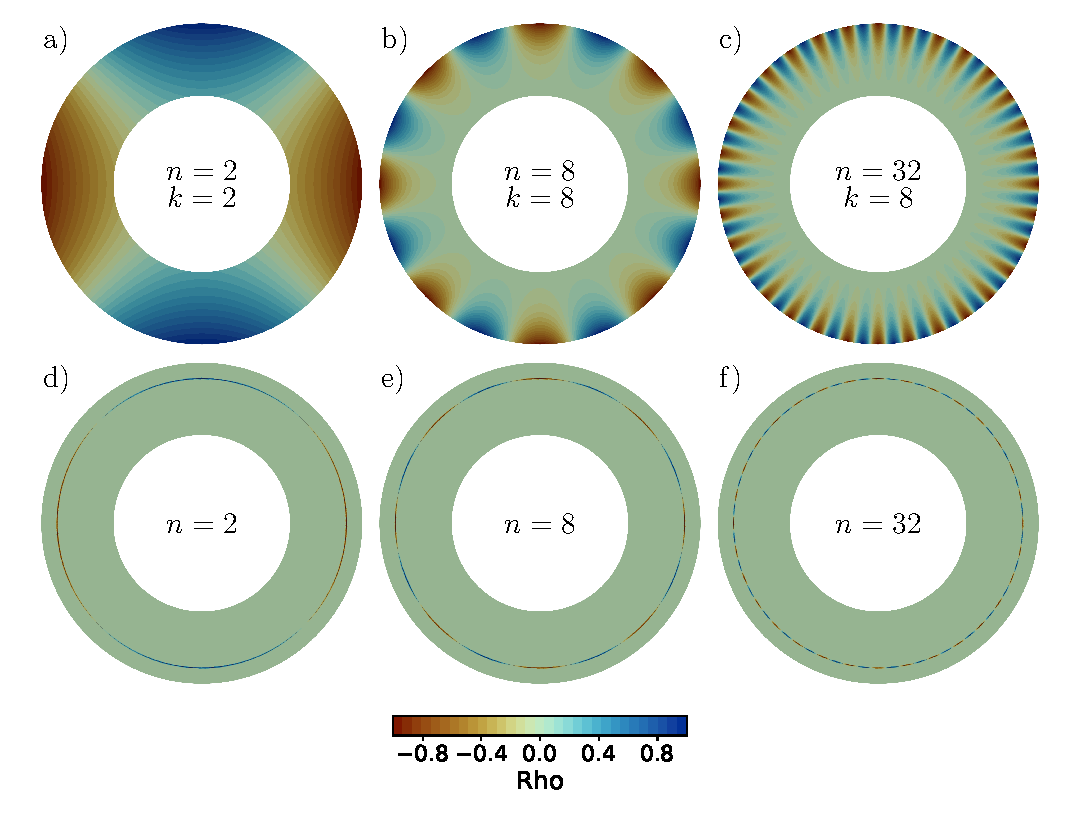
\includegraphics[
    width=\linewidth,
    height=\TopRowFigureHeight,
    keepaspectratio
  ]{../annulus/kramer/figure_1_kramer_annulus_rho_ana.pdf}
\end{minipage}

\vspace{0.1in}

\noindent
\begin{minipage}[t]{0.475\textwidth}
  \centering
  \PanelTitle{Thieulot spherical shell}
  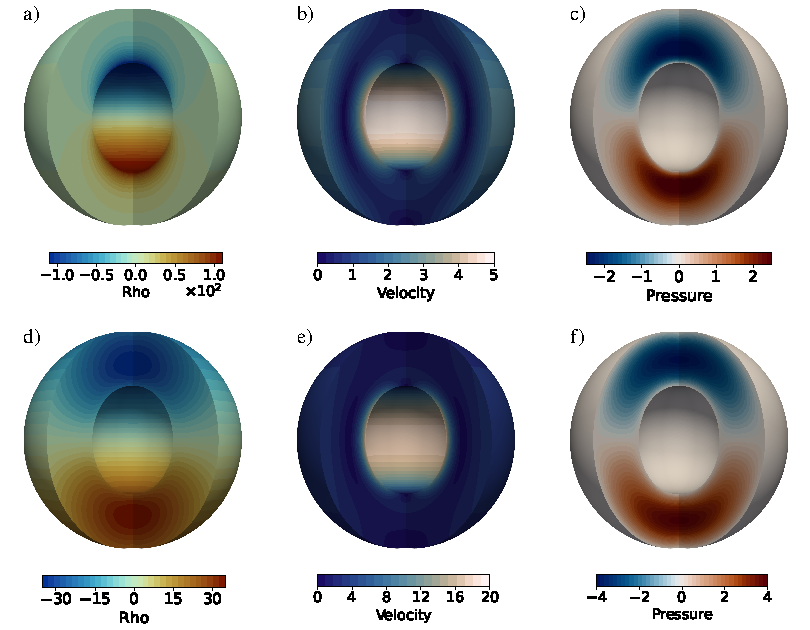
\includegraphics[
    width=\linewidth,
    height=\BottomRowFigureHeight,
    keepaspectratio
  ]{../spherical/thieulot/figure_2_thieulot_analytical.pdf}
\end{minipage}
\ColumnGap
\begin{minipage}[t]{0.475\textwidth}
  \centering
  \PanelTitle{Kramer spherical shell}
  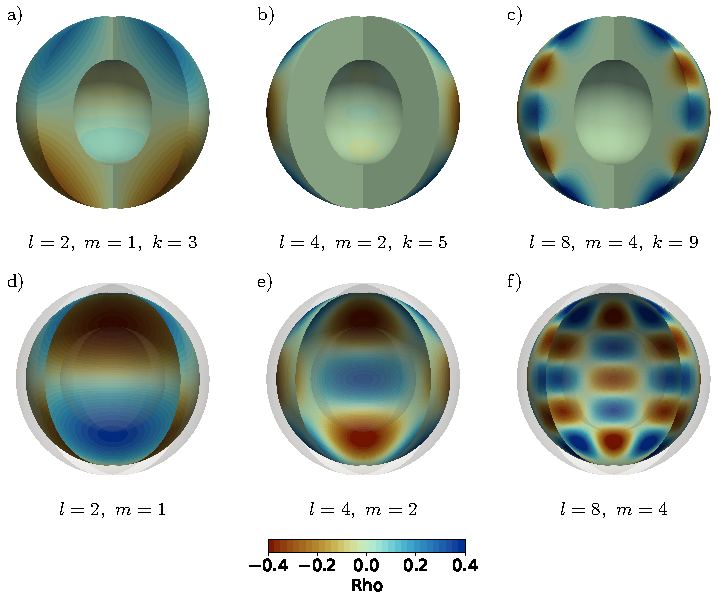
\includegraphics[
    width=\linewidth,
    height=\BottomRowFigureHeight,
    keepaspectratio
  ]{../spherical/kramer/figure_2_kramer_rho_ana.pdf}
\end{minipage}

\end{document}
